\documentclass{scrartcl} % scrartcl of scrreprt
% Include all project wide packages here.
\usepackage{fullpage}
\usepackage{polyglossia}
\setmainlanguage{dutch}
\usepackage{csquotes}
\usepackage{graphicx}
\usepackage{epstopdf}
\usepackage{pdfpages}
\usepackage{caption}
\usepackage[list=true]{subcaption}
\usepackage{float}
%\usepackage{mathtools}
\usepackage{standalone}
\usepackage{import}
\usepackage{tocloft}
\usepackage{wrapfig}
\usepackage{authblk}
\usepackage{array}
\usepackage{booktabs}
\usepackage[toc,page,title,titletoc]{appendix}
\usepackage{xunicode}
\usepackage{amsmath}
\usepackage{fontspec}
\usepackage{unicode-math}
\usepackage[
    backend=bibtexu,
	texencoding=utf8,
bibencoding=utf8,
    style=ieee,
    sortlocale=nl_NL,
    language=auto
]{biblatex}
\usepackage{listings}
\newcommand{\includecode}[3][c]{\lstinputlisting[caption=#2, escapechar=, style=#1]{#3}}
\newcommand{\superscript}[1]{\ensuremath{^{\textrm{#1}}}}
\newcommand{\subscript}[1]{\ensuremath{_{\textrm{#1}}}}


\newcommand{\chapternumber}{\thechapter}
\renewcommand{\appendixname}{Bijlage}
\renewcommand{\appendixtocname}{Bijlagen}
\renewcommand{\appendixpagename}{Bijlagen}

\usepackage[hidelinks]{hyperref} %<--------ALTIJD ALS LAATSTE

\renewcommand{\familydefault}{\sfdefault}

\setmainfont[Ligatures=TeX]{Myriad Pro}
\setmathfont{Asana Math}
\setmonofont{Lucida Console}

\usepackage{titlesec, blindtext, color}
\definecolor{gray75}{gray}{0.75}
\newcommand{\hsp}{\hspace{20pt}}
\titleformat{\chapter}[hang]{\Huge\bfseries}{\chapternumber\hsp\textcolor{gray75}{|}\hsp}{0pt}{\Huge\bfseries}
\renewcommand{\familydefault}{\sfdefault}
\renewcommand{\arraystretch}{1.2}
\setlength\parindent{0pt}

%For code listings
\definecolor{black}{rgb}{0,0,0}
\definecolor{browntags}{rgb}{0.65,0.1,0.1}
\definecolor{bluestrings}{rgb}{0,0,1}
\definecolor{graycomments}{rgb}{0.4,0.4,0.4}
\definecolor{redkeywords}{rgb}{1,0,0}
\definecolor{bluekeywords}{rgb}{0.13,0.13,0.8}
\definecolor{greencomments}{rgb}{0,0.5,0}
\definecolor{redstrings}{rgb}{0.9,0,0}
\definecolor{purpleidentifiers}{rgb}{0.01,0,0.01}


\lstdefinestyle{csharp}{
language=[Sharp]C,
showspaces=false,
showtabs=false,
breaklines=true,
showstringspaces=false,
breakatwhitespace=true,
escapeinside={(*@}{@*)},
columns=fullflexible,
commentstyle=\color{greencomments},
keywordstyle=\color{bluekeywords}\bfseries,
stringstyle=\color{redstrings},
identifierstyle=\color{purpleidentifiers},
basicstyle=\ttfamily\small}

\lstdefinestyle{c}{
language=C,
showspaces=false,
showtabs=false,
breaklines=true,
showstringspaces=false,
breakatwhitespace=true,
escapeinside={(*@}{@*)},
columns=fullflexible,
commentstyle=\color{greencomments},
keywordstyle=\color{bluekeywords}\bfseries,
stringstyle=\color{bluestrings},
identifierstyle=\color{purpleidentifiers}
}

\lstdefinestyle{vhdl}{
language=VHDL,
showspaces=false,
showtabs=false,
breaklines=true,
showstringspaces=false,
breakatwhitespace=true,
escapeinside={(*@}{@*)},
columns=fullflexible,
commentstyle=\color{greencomments},
keywordstyle=\color{bluekeywords}\bfseries,
stringstyle=\color{redstrings},
identifierstyle=\color{purpleidentifiers}
}

\lstdefinestyle{xaml}{
language=XML,
showspaces=false,
showtabs=false,
breaklines=true,
showstringspaces=false,
breakatwhitespace=true,
escapeinside={(*@}{@*)},
columns=fullflexible,
commentstyle=\color{greencomments},
keywordstyle=\color{redkeywords},
stringstyle=\color{bluestrings},
tagstyle=\color{browntags},
morestring=[b]",
  morecomment=[s]{<?}{?>},
  morekeywords={xmlns,version,typex:AsyncRecords,x:Arguments,x:Boolean,x:Byte,x:Char,x:Class,x:ClassAttributes,x:ClassModifier,x:Code,x:ConnectionId,x:Decimal,x:Double,x:FactoryMethod,x:FieldModifier,x:Int16,x:Int32,x:Int64,x:Key,x:Members,x:Name,x:Object,x:Property,x:Shared,x:Single,x:String,x:Subclass,x:SynchronousMode,x:TimeSpan,x:TypeArguments,x:Uid,x:Uri,x:XData,Grid.Column,Grid.ColumnSpan,Click,ClipToBounds,Content,DropDownOpened,FontSize,Foreground,Header,Height,HorizontalAlignment,HorizontalContentAlignment,IsCancel,IsDefault,IsEnabled,IsSelected,Margin,MinHeight,MinWidth,Padding,SnapsToDevicePixels,Target,TextWrapping,Title,VerticalAlignment,VerticalContentAlignment,Width,WindowStartupLocation,Binding,Mode,OneWay,xmlns:x}
}

%defaults
\lstset{
basicstyle=\ttfamily\small,
extendedchars=false,
numbers=left,
numberstyle=\ttfamily\tiny,
stepnumber=1,
tabsize=4,
numbersep=5pt
}
\addbibresource{../../library/bibliography.bib}

\title{EPO3: Eindrapport - Instructiedecoder}
\author{Robin Hes}

\begin{document}
\chapter{Instructiedecoder}
\label{ch:decoder}
%specs
\subsection{Specificaties}
De decoder accepteert een vaste set instructies, zoals in tabel \ref{tab:decoder-instruction}

\begin{table}[H]
	\centering
	\caption{Door de decoder ondersteunde instructies}
	\label{tab:decoder-instruction}
	\begin{tabular}{c c c p{0.5\textwidth}}
		\hline\hline
		Code & Naam & Interne naam & Beschrijving \\
		\hline
		000 & Switch & i\_switch & Schakelt over naar het andere screen buffer \\
		001 & Fill & i\_fill & Schakelt de draw-rect module in om het gehele scherm naar de gegeven kleur te vullen \\
		010 & Draw pixel & i\_pixel & Schakelt de draw-pixel module in om op de gegeven coördinaten een pixel te tekenen, met de gegeven kleur \\
		011 & Draw rectangle & i\_rect & Schakelt de draw-rect module in om op de gegeven coördinaten een rechthoek te tekenen met de gegeven kleur, breedte en hoogte \\
		100 & Draw filled rectangle & i\_frect & Schakelt de draw-filled-rect module in om op de gegeven coördinaten een gevulde rechthoek te tekenen, met de gegeven kleur, breedte en hoogte \\
		101 & Draw line & i\_line & Schakelt de draw-line module in om een lijn te tekenen van de eerste gegeven coördinaten naar de tweede gegeven coördinaten, met de gegeven kleur \\
		110 & Draw sprite & i\_sprite & Schakelt de draw-sprite module in om een sprite te tekenen op de gegeven coördinaten, met de gegeven kleur \\
		111 & Load sprite & i\_lsprite & Laadt de gegeven sprite in het VRAM rechthoek te tekenen met de gegeven kleur, breedte en hoogte \\
		\end{tabular}
\end{table}
\small
Een specificatie per instructie (het protocol) is gegeven in bijlage \ref{app:instructies}.
\\\\
Deze instructies komen binnen over de SPI-interface. Wanneer het signaal spi\_data\_available omhoog gaat, dient de decoder de data uit spi\_data\_rx te lezen en te interpreteren als een nieuwe instructie (zie tabel \ref{tab:decoder-instruction}) of data die bij de huidige instructie hoort.
Wanneer er sprites geladen moeten worden dient de decoder de inkomende sprite-data (ramdata) weg te schrijven naar de correcte plaats in het VRAM (ramaddr), mits hij daar toegang toe heeft (decoder\_can\_access). Wanneer hij deze data gaat schrijven, dienen de signalen decoder\_write en decoder\_claim hoog te zijn. Het laden van sprites kan alleen direct na een reset. Bij het binnenkomen van de eerste instructie anders dan load sprite dient het signaal is\_init op laag gezet te worden, om aan te geven dat alle sprites geladen zijn.
Als de decoder een draw-instructie binnen krijgt, dient hij de daarop volgende data op de correcte uitgangen te zetten en als laatst het correcte enable-bit (en) op hoog te zetten.
Bij het verwerken van de switch-instructie, moet het signaal asb geïnverteerd worden, maar alleen als het signaal vga\_vsync hoog is. Dit voorkomt screen tearing.
Als laatste, wanneer decoder en de rest van de GPU klaar zijn voor een nieuwe instructie, bijvoorbeeld na het laden van een sprite, een switch of wanneer het signaal draw\_ready hoog wordt, dient de decoder alle draw-modules uit te schakelen en de CPU in te lichten dat hij klaar is, door het signaal int\_ready hoog te maken.
De hierboven beschreven in- en uitgangen staan als blokschema uitgewerkt in figuur \ref{fig:decoder-schema}. De workflow van de decoder zoals beschreven is schematisch weergegeven in figuur \ref{fig:decoder-flow}.

\begin{figure}[H]
	\centering
	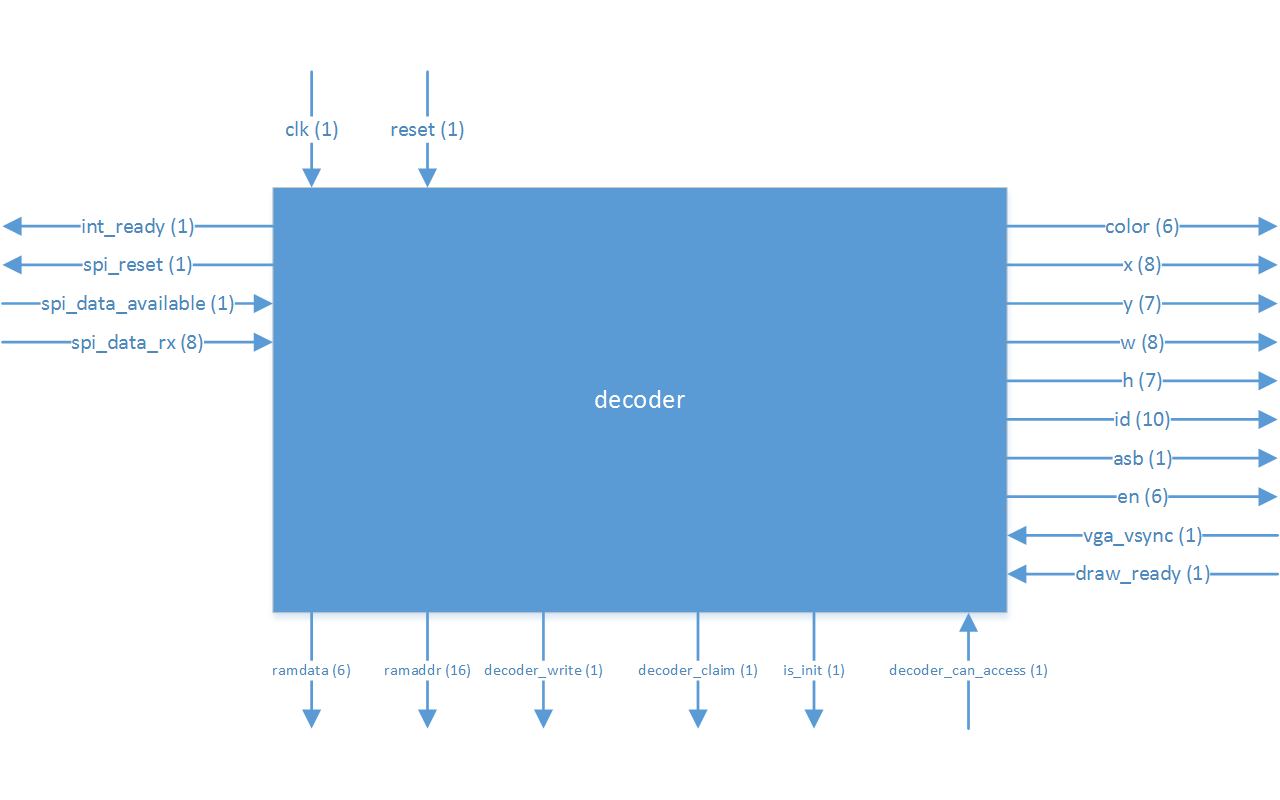
\includegraphics[width=\textwidth]{resource/decoder.png}
	\caption{Een blokschema van de decoder, met de namen van de gebruikte in- en uitgangen en tussen haakjes het aantal bits}
	\label{fig:decoder-schema}
\end{figure}

\begin{figure}[H]
	\centering
	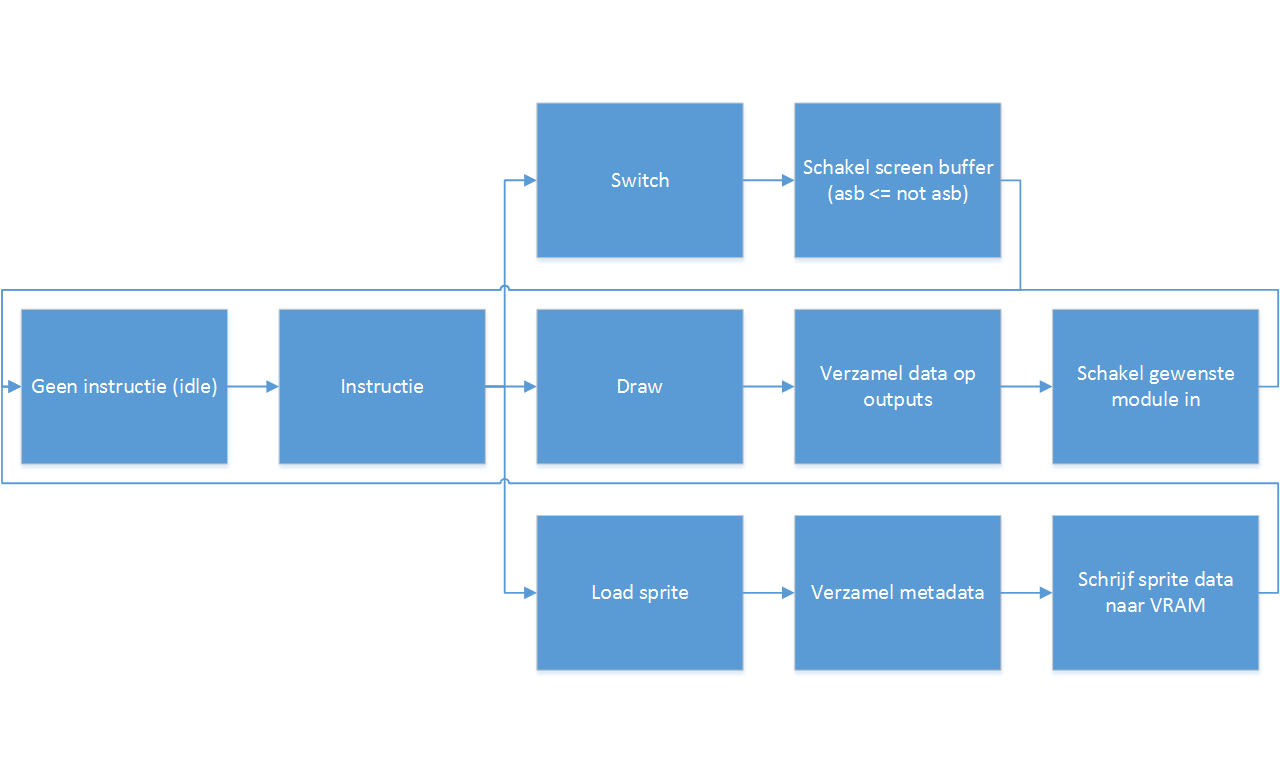
\includegraphics[width=\textwidth]{resource/decoder-flow.png}
	\caption{De workflow van de decoder}
	\label{fig:decoder-flow}
\end{figure}

%VHDL
\subsection{Ontwerp en implementatie}
De decoder is geïmplementeerd als een FSM. Het sequentiële deel van de FSM vernieuwt uiteraard alleen de (state) registers, waar het combinatorische gedeelte van de schakeling de daadwerkelijke instructieverwerking op zich neemt. In dit combinatorische gedeelte wordt afhankelijk van de huidige instructie, welke uit het eerste byte wat binnen komt over de SPI wordt afgeleid, en het huidige SPI-packet number bepaald wat voor informatie er ontvangen is. De instructie (current\_instruction) en het pakketnummer (packet\_num) zijn de state variabelen van de FSM. Wanneer er nog geen instructie geladen is, gebruikt de decoder het eerst volgende inkomende pakket om de volgende instructie uit te lezen. Wanneer de instructie bekend is, wordt met een counter het nummer van de daaropvolgende bytes bijgehouden. Deze bytes worden dan geïnterpreteerd afhankelijk van de huidige instructie en het pakketnummer. Wanneer het pakketnummer gelijk is aan het aantal pakketten dat bij een instructie hoort, onderneemt de decoder de benodigde actie, zoals het inschakelen van de juiste draw-module, en reset hij zichzelf daarna naar een state waarin hij wacht op de volgende instructie. Dit proces wordt op deze manier constant herhaald, wanneer de GPU ingeschakeld is.
\\\\
Bij het laden van sprites ontvangt de decoder alle relevante gegevens over die sprite (metadata). Deze metadata bestaat uit de breedte in pixels van de sprite, het aantal pakketten sprite-data wat ontvangen moet worden en een identificatienummer (id). Als deze informatie binnen is, wordt de sprite per zes bits weggeschreven naar het VRAM. Het te schrijven adres bestaat uit het id van de sprite, plus de waarde van een interne counter die het nummer van het huidige datablok bijhoudt.
\\
Wanneer er een draw-instructie binnenkomt verzamelt de decoder eerst alle informatie betreffende deze instructie, door deze gebufferd aan zijn uitgang te zetten. Hierbij moet gedacht worden aan de bijvoorbeeld x, y en kleur, afhankelijk van wat er getekend moet worden. Wanneer al deze data ontvangen is schakelt de decoder de correcte draw-module in door, het juiste bit in het enable-uitgangssignaal (en) hoog te maken.
\\
Wanneer de switch-instructie binnenkomt, wordt het signaal asb geïnverteerd en is de decoder meteen klaar.
\\
\\
Zoals al vermeld bij SPI, zijn we er helaas niet in geslaagd om een helemaal correct functionerende SPI-interface te maken, om onbekende reden. Omdat de decoder direct afhankelijk is van de SPI-interface, loopt deze vast op het moment dat de SPI-module faalt. Om er voor te zorgen dat de decoder daarna zonder de hele GPU te resetten toch weer verder gaat, hebben we een timer ingebouwd die de SPI-module en de decoder ``soft-reset'', zodra deze afgelopen is. In de praktijk levert dit een zo nu en dan knipperend beeld en soms artifacts op, maar dat is beter dan een beeld dat steeds bevriest. Naast deze maatregel resetten we de SPI-module ook na iedere ontvangen instructie

%VHDL simulatie
\subsection{VHDL simulatie}
In ModelSim is een testbench gebruikt die verschillend bytes aan de ingang van de decoder zet, om te zien of de decoder ze omzet naar de juiste instructie en data.
\\\\
Als eerst wordt een sprite naar het VRAM geladen. In figuur \ref{fig:decoder-modelsim-lsprite} is te zien hoe de met spi\_data\_available de inkomende data naar het VRAM geschreven wordt. Wanneer het laatste pakket ontvangen wordt (nummer 4, zoals opgeslagen in x), heeft de counter (opgeslagen in h) dit aantal bereikt en bemerkt de decoder dat hij klaar is en gaat int\_ready omhoog.

\begin{figure}[H]
	\centering
	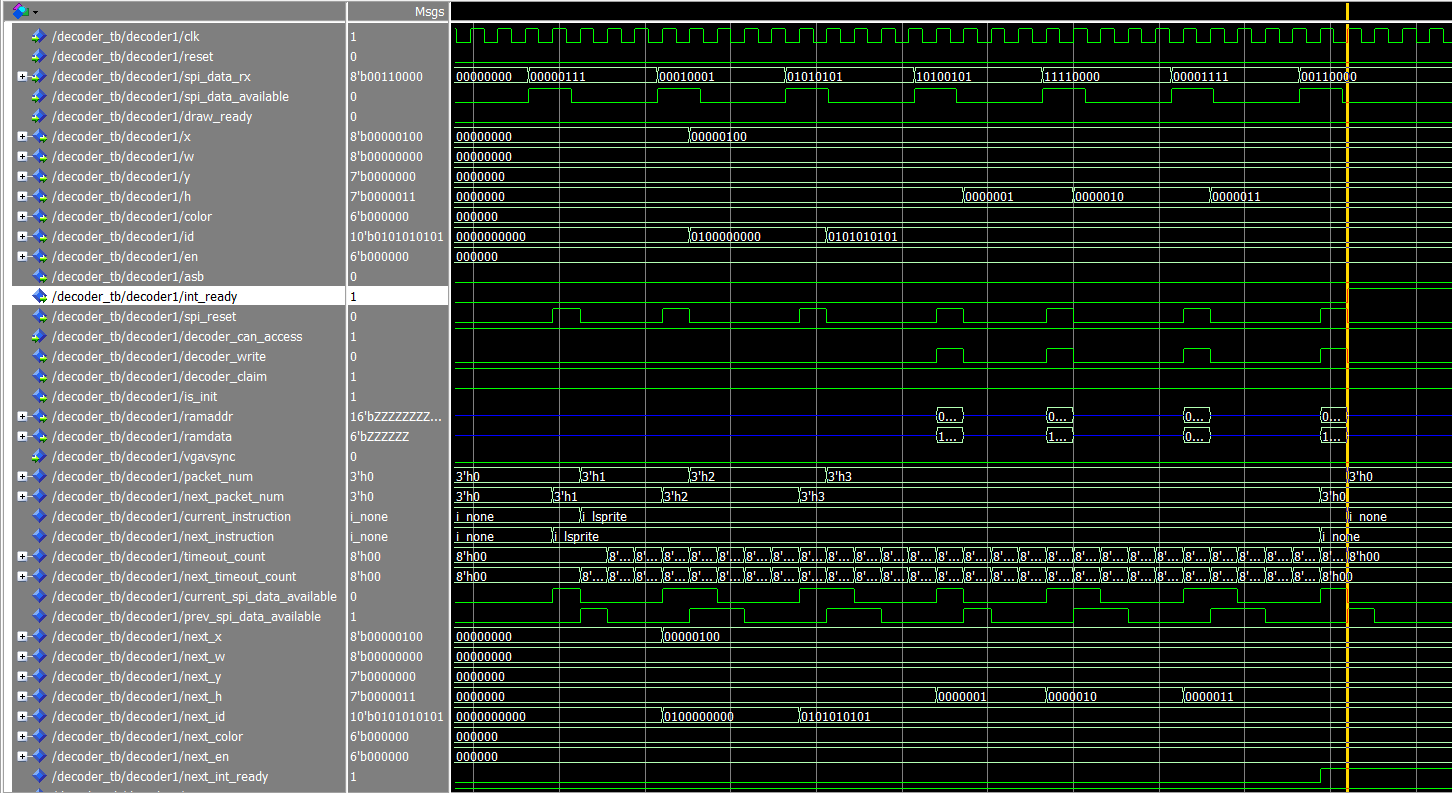
\includegraphics[width=\textwidth]{resource/decoder-modelsim-lsprite.png}
	\caption{Een fragment van de decoder waveform, waarin een sprite naar het VRAM geladen wordt}
	\label{fig:decoder-modelsim-lsprite}
\end{figure}

Vervolgens wordt een rechthoek getekend, het gedeelte van de waveform waarin dit gebeurt is te zien in figuur \ref{fig:decoder-modelsim-rect}. Te zien is dat color, x (x0), y (y0), w (x1) h (y1) op de juiste uitgangen worden gezet en dat vervolgens en(1) hoog wordt om draw\_rect te activeren.

\begin{figure}[H]
	\centering
	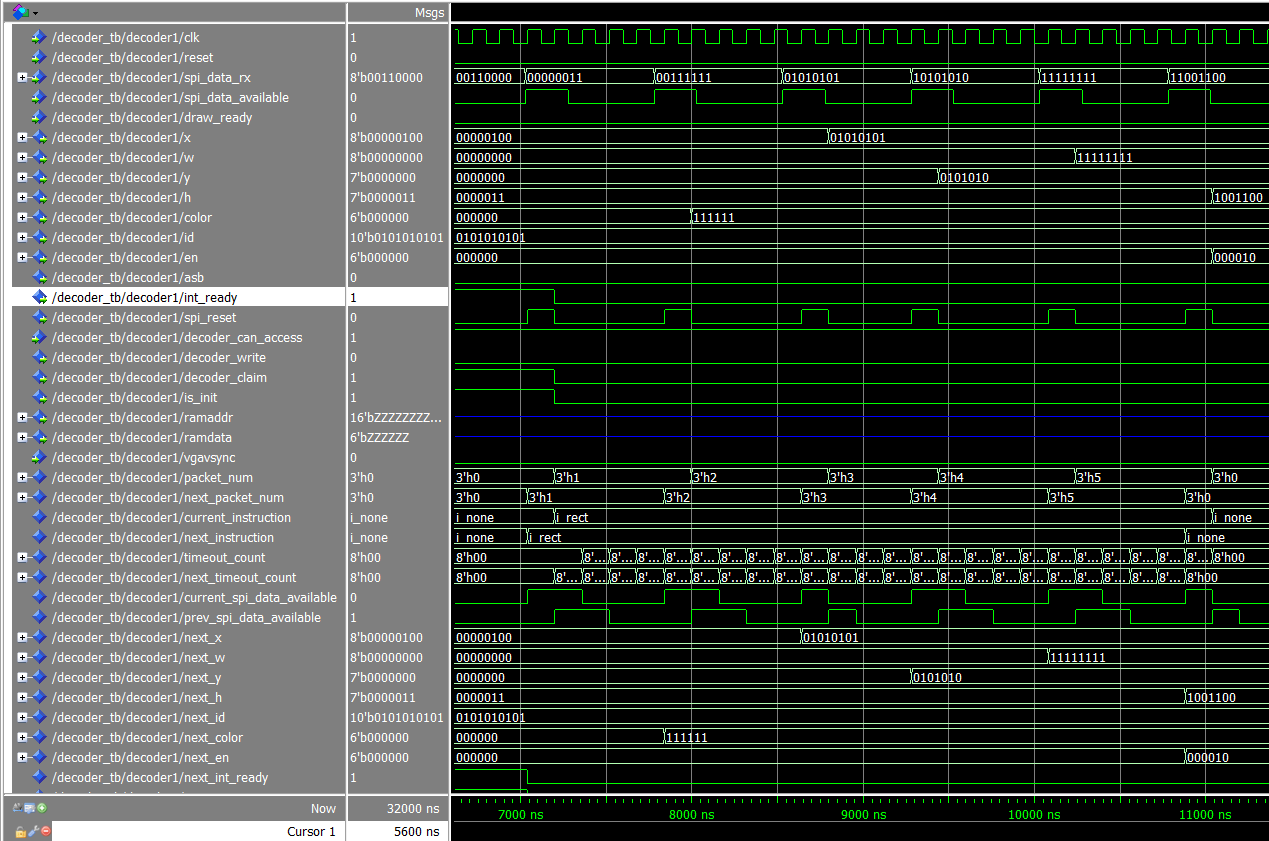
\includegraphics[width=\textwidth]{resource/decoder-modelsim-rect.png}
	\caption{Een fragment van de decoder waveform, waarin een rectangle getekend wordt}
	\label{fig:decoder-modelsim-rect}
\end{figure}

Even later wordt gesimuleerd dat draw\_rect zijn done-signaal hoog maakt (in de decoder heet dit signaal draw\_ready). De decoder moet dit signaal doorgeven naar de CPU, door middel van int\_ready. In figuur \ref{fig:decoder-modelsim-draw-ready} is te zien dat dit ook daadwerkelijk gebeurt.

\begin{figure}[H]
	\centering
	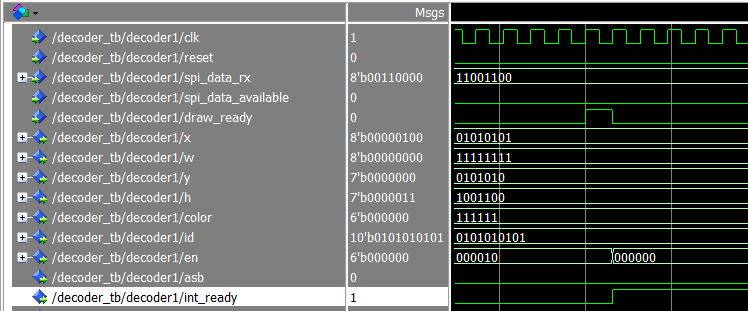
\includegraphics[width=\textwidth]{resource/decoder-modelsim-draw-ready.png}
	\caption{Een fragment van de decoder waveform, waarin draw\_ready hoog wordt}
	\label{fig:decoder-modelsim-draw-ready}
\end{figure}

De andere draw-modules worden op vergelijkbare manier aangestuurd en zijn allemaal werkend getest.

Als laatst testen we de switch-instructie, waarin het screen buffer wordt gewisseld. In de waveform in figuur \ref{fig:decoder-modelsim-switch} is te zien dat het signaal asb inderdaad geïnverteerd wordt bij het binnenkomen van de switch-instructie. Vervolgens geeft de decoder netjes aan dat hij klaar is voor de volgende instructie, door middel van het signaal int\_ready.

\begin{figure}[H]
	\centering
	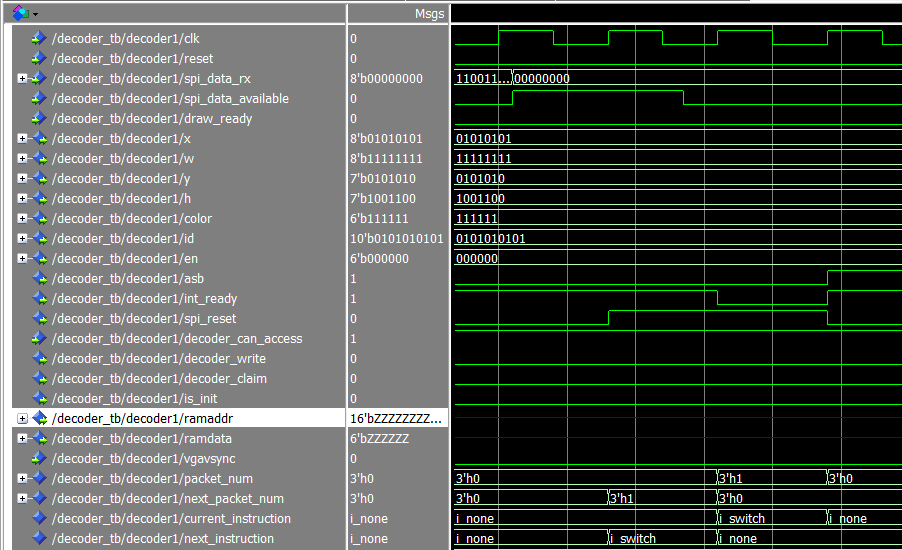
\includegraphics[width=\textwidth]{resource/decoder-modelsim-switch.png}
	\caption{Een fragment van de decoder waveform, waarin van schermbuffer gewisseld wordt}
	\label{fig:decoder-modelsim-switch}
\end{figure}

Uit deze drie tests mag geconcludeerd worden dat de decoder alle vereiste instructies kan verwerken. Ook de timeout is werkend getest en in de praktijk blijkt dat deze timer inderdaad zorgt dat de GPU niet meer vast loopt.

%Synthese
\subsection{Synthese}
De decoder is een vrij omvangrijke module, hij slaat alle input die benodigd is voor de draw-modules op in registers en bevat daarnaast de nodige arithmiek voor het schrijven van sprites naar het VRAM en voor het optellen van de failsafe-counter. Deze registers en arithmiek resulteren in een groot gebruikt chipoppervlak. Synthese met compile\_ultra levert een totaal celloppervlak op van 3139 transistoren. Handmatige plaatsing van de cellen op 20 rijen met een onderlinge afstand van 7 en de optie ``vary distance'' uitgeschakeld, levert met Trout een lay-out op met een totaal van 22440 transistoren op, waarvan er 6285 daadwerkelijk worden gebruikt. Een efficiëntie van 28.01\% dus.

%Switchlevel test
\subsection{Switch-level simulatie}
Zowel circuit als lay-out zijn gesimuleerd met SLS en vervolgens vergeleken met de originele ModelSim testbench. Beide keren leverde dit een correct resultaat op.

%Conclusie
\subsection{Conclusie}
Wanneer de decoder de juiste data binnen krijgt over de SPI-interface, functioneert hij geheel correct. Helaas is dit niet altijd het geval en hebben we maatregelen moeten treffen om hier omheen te werken. Dit, en het feit dat de decoder sowieso al een vrij complexe module is, heeft er voor gezorgd dat de decoder de een-na-grootste module in de GPU is. Een andere aanpak was geweest om de decoder op te splitsen in twee of meerdere delen en/of losse componenten op te delen. Op deze manier zouden de verschillende registers en/of adders eventueel ook nog kunnen worden hergebruikt.

\end{document}
